\documentclass[12pt,a4paper]{article}
\usepackage{amsmath}
\usepackage{graphicx}
\usepackage{float}
\usepackage{listings}
\usepackage{xcolor}
\usepackage{tikz}
\usepackage{comment}
\usetikzlibrary{shapes.geometric, arrows}

% Define colors for the listings
\definecolor{codegray}{gray}{0.9}
\definecolor{codegreen}{rgb}{0,0.6,0}
\definecolor{codeblue}{rgb}{0,0,0.6}

% Listing settings
\lstset{
    backgroundcolor=\color{codegray},
    commentstyle=\color{codegreen},
    keywordstyle=\color{codeblue},
    numberstyle=\tiny\color{gray},
    stringstyle=\color{magenta},
    basicstyle=\ttfamily\footnotesize,
    breakatwhitespace=false,
    breaklines=true,
    captionpos=b,
    keepspaces=true,
    numbers=left,
    numbersep=5pt,
    showspaces=false,
    showstringspaces=false,
    showtabs=false,
    tabsize=2,
    language=Python
}

% TikZ settings for flowchart
\tikzstyle{startstop} = [rectangle, rounded corners, minimum width=3cm, minimum height=1cm,text centered, draw=black, fill=red!30]
\tikzstyle{process} = [rectangle, minimum width=3cm, minimum height=1cm, text centered, draw=black, fill=orange!30]
\tikzstyle{decision} = [diamond, minimum width=3cm, minimum height=1cm, text centered, draw=black, fill=green!30]
\tikzstyle{arrow} = [thick,->,>=stealth]
\title{Shear Force and Bending Moment Analysis of a Beam Under Moving Load Using Influence Line Diagrams}
\author{Harshit}
\date{\today}

\begin{document}
\maketitle

\section*{Objective}
To develop a Python-based program to calculate the shear force and bending moment for a simply supported beam under a moving load using the influence line diagram concept.

\section*{Problem Statement}
A simply supported beam is subjected to two moving point loads \( W_1 \) and \( W_2 \), spaced by a distance \( x \). The program must:
\begin{itemize}
    \item Accept user-defined values for beam length \( L \), loads \( W_1 \) and \( W_2 \), and spacing \( x \)
    \item Calculate:
    \begin{itemize}
        \item Maximum reactions at supports A and B
        \item Bending moment \( BM_{01} \) when \( W_1 \) is at \( 0 \) m
        \item Shear force \( SF_{01} \) at mid-span (\( 0.5L \))
        \item Maximum shear force \( SF_{\text{max}} \) and its location \( y \)
        \item Maximum bending moment \( BM_{\text{max}} \) and its location \( z \)
    \end{itemize}
\end{itemize}

\section*{Inputs}
\begin{itemize}
    \item Length of beam: \( L \, \text{m} \)
    \item Load values: \( W_1 \, \text{kN}, \, W_2 \, \text{kN} \)
    \item Distance between loads: \( x \, \text{m} \)
\end{itemize}

\section*{Methodology}
We use influence line theory to determine the variation of support reactions, shear force, and bending moment due to moving loads. The beam is analyzed at multiple positions of the moving loads to capture critical values.

\subsection*{Reaction Influence Lines}
For a simply supported beam:
\[
R_A = \frac{L - a}{L}, \quad R_B = \frac{a}{L}
\]
where \( a \) is the position of the point load from A.

\subsection*{Shear Force Influence Line at Point \( p \)}
\[
IL_{SF}(x) = 
\begin{cases}
\frac{L - p}{L}, & \text{if } x < p \\
-\frac{p}{L}, & \text{if } x > p \\
\text{undefined}, & \text{if } x = p
\end{cases}
\]

\subsection*{Bending Moment Calculation}
\[
BM(p) = R_A \cdot p - \sum (w_i \cdot (p - a_i)), \quad \text{for } a_i < p
\]

\section{Design Calculations}

\subsection*{Given Data}
\begin{itemize}
    \item Length of Beam, $L = \textbf{...}~\text{m}$
    \item Load 1, $W_1 = \textbf{...}~\text{kN}$
    \item Load 2, $W_2 = \textbf{...}~\text{kN}$
    \item Distance between Loads, $x = \textbf{...}~\text{m}$
\end{itemize}

\subsection*{Step 1: Maximum Reactions at Supports}
\begin{align*}
\text{Using Influence Line Diagram (ILD):} \\
R_A^{\max} &= \max_{position} \left( W_1 \cdot \frac{L - a}{L} + W_2 \cdot \frac{L - (a + x)}{L} \right) \\
R_B^{\max} &= \max_{position} \left( W_1 \cdot \frac{a}{L} + W_2 \cdot \frac{a + x}{L} \right)
\end{align*}

\subsection*{Step 2: Bending Moment at $W_1 = 0$ m}
\begin{align*}
BM_{01} &= R_B \cdot L \\
\text{(All the load acts at left support, so moment about A is zero, and max at B)}
\end{align*}

\subsection*{Step 3: Shear Force at Mid-span}
\begin{align*}
SF_{0.5L} &= R_A - \sum W_i \quad \text{(where $W_i$ are to the left of mid-span)}
\end{align*}

\subsection*{Step 4: Maximum Bending Moment and Shear Force}
\begin{align*}
BM_{\max} &= \max_{positions} \left( R_A \cdot a - W_1 \cdot (a - d_1) - W_2 \cdot (a - d_2) \right) \\
SF_{\max} &= \max_{positions} \left| R_A - \sum W_i \right|
\end{align*}
\begin{itemize}
    \item $a$ = location from support A
    \item $d_1$, $d_2$ = distances of $W_1$, $W_2$ from point of interest
\end{itemize}

\subsection*{Step 5: Final Results}
\begin{itemize}
    \item Maximum Reaction at A: $\boxed{R_A^{\max} = \textbf{...}~\text{kN}}$
    \item Maximum Reaction at B: $\boxed{R_B^{\max} = \textbf{...}~\text{kN}}$
    \item Bending Moment at $W_1 = 0$: $\boxed{BM_{01} = \textbf{...}~\text{kNm}}$
    \item Shear Force at mid-span: $\boxed{SF_{0.5L} = \textbf{...}~\text{kN}}$
    \item Maximum Shear Force: $\boxed{SF_{\max} = \textbf{...}~\text{kN at } y~\text{m from A}}$
    \item Maximum Bending Moment: $\boxed{BM_{\max} = \textbf{...}~\text{kNm at } z~\text{m from A}}$
\end{itemize}

\section{Outcomes}

The analysis of a simply supported beam subjected to a moving load using the Influence Line Diagram (ILD) approach led to the following key outcomes:

\begin{itemize}
    \item Successfully calculated the maximum reactions at supports A and B based on the relative positions of moving loads.
    \item Accurately computed the bending moment at the start of the beam ($W_1 = 0$ m) and the shear force at the midpoint of the beam.
    \item Determined the maximum bending moment and shear force values along with their positions from support A, which are critical for structural design.
    \item Developed a modular and well-commented Python program capable of simulating moving load effects using influence lines, shear force and bending moment envelopes.
    \item Enabled easy visualization of loading, shear force, bending moment diagrams, and ILD using matplotlib.
\end{itemize}

This implementation aids in optimizing structural design by identifying critical points under dynamic loading conditions, thus ensuring safer and more cost-effective engineering solutions.


\section*{Code Structure}
\begin{itemize}
    \item \textbf{analyze\_ss\_movingload.py}: Main module that coordinates analysis and outputs results.
    \item \textbf{influence\_line.py}: Contains influence line logic and envelope calculation methods.
    \item \textbf{visualization.py}: Responsible for plotting beam, shear force, and bending moment diagrams.
    \item \textbf{beam\_calculator.py}: (Optional) Modular functions to support calculations.
\end{itemize}

\section{Solution in Python}
\lstinputlisting{analyze_ss_movingload.py}

\section{Flowchart}
\usetikzlibrary{shapes.geometric, arrows.meta, positioning}

\tikzstyle{startstop} = [rectangle, rounded corners, minimum width=3cm, minimum height=1cm,text centered, draw=black, fill=blue!20]
\tikzstyle{process} = [rectangle, minimum width=4cm, minimum height=1cm, text centered, draw=black, fill=green!20]
\tikzstyle{decision} = [diamond, aspect=2, draw=black, fill=orange!30, text centered, inner sep=1pt]
\tikzstyle{arrow} = [thick, ->, >=stealth]


\begin{tikzpicture}[node distance=1.3cm and 1cm]

\node (start) [startstop] {Start};
\node (input) [process, below=of start] {Take Inputs: $L$, $W_1$, $W_2$, $x$};
\node (init) [process, below=of input] {Initialize Beam and Load Positions};
\node (loop) [process, below=of init] {Loop: For all load positions};
\node (reaction) [process, below=of loop] {Calculate Reactions using Influence Lines};
\node (shear) [process, below=of reaction] {Compute Shear Force at Mid-span};
\node (moment) [process, below=of shear] {Compute Bending Moment};
\node (update) [process, below=of moment] {Update Max SF and BM if Needed};
\node (bm0) [process, below=of update] {Compute BM at $W_1 = 0$};
\node (display) [process, below=of bm0] {Display Results and Plot Graphs};
\node (end) [startstop, below=of display] {End};

\draw [arrow] (start) -- (input);
\draw [arrow] (input) -- (init);
\draw [arrow] (init) -- (loop);
\draw [arrow] (loop) -- (reaction);
\draw [arrow] (reaction) -- (shear);
\draw [arrow] (shear) -- (moment);
\draw [arrow] (moment) -- (update);
\draw [arrow] (update) -- (bm0);
\draw [arrow] (bm0) -- (display);
\draw [arrow] (display) -- (end);
\end{tikzpicture}
\section*{Visualizations}
\begin{itemize}
    \item Influence Line for Reactions at A and B
    \item Influence Line for Shear Force at \( p \)
    \item Shear Force Envelope
    \item Bending Moment Envelope
\end{itemize}

\begin{center}
    
\includegraphics[width=1.5\textwidth]{Figure_2.png}
    
    \vspace{1em}
    
    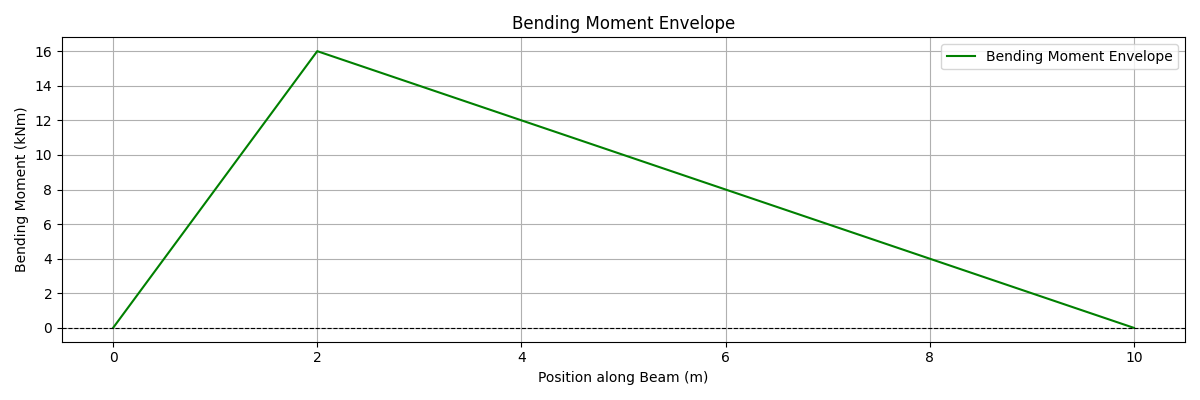
\includegraphics[width=1.0\textwidth]{Figure_11.png}

    \vspace{1em}

    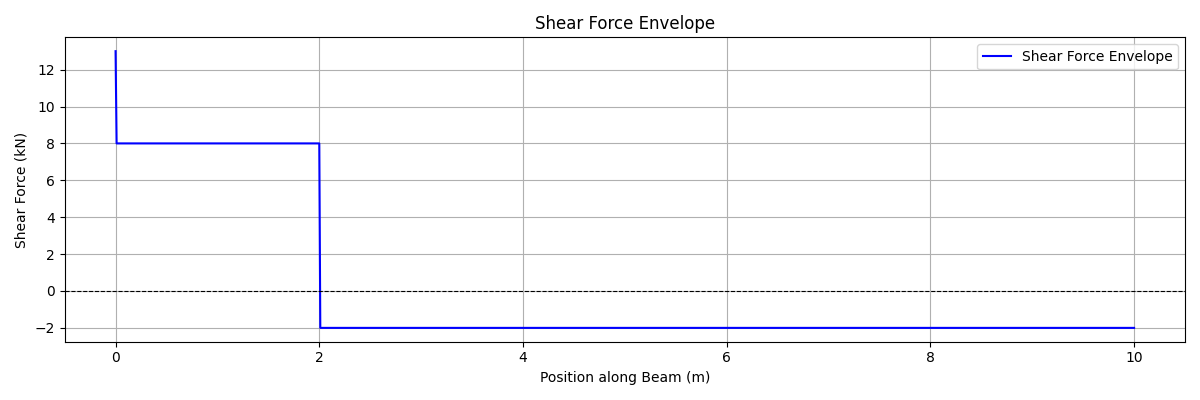
\includegraphics[width=1.0\textwidth]{Figure_1.png}

\end{center}

\section*{Results}

The results of the beam analysis under a moving load using the Influence Line Diagram (ILD) method are as follows:

\begin{itemize}
    \item \textbf{Maximum Reaction at Support A:} $R_A = \texttt{<value>} \, \text{kN}$
    \item \textbf{Maximum Reaction at Support B:} $R_B = \texttt{<value>} \, \text{kN}$
    \item \textbf{Bending Moment at } $W_1 = 0 \, \text{m}: \quad M_{W_1=0} = \texttt{<value>} \, \text{kNm}$
    \item \textbf{Shear Force at Mid-span} $\left(x = \frac{L}{2}\right): \quad V_{x = L/2} = \texttt{<value>} \, \text{kN}$
    \item \textbf{Maximum Shear Force:} $V_{\text{max}} = \texttt{<SF\_max>} \, \text{kN} \quad \text{at} \quad y = \texttt{<location>} \, \text{m}$
    \item \textbf{Maximum Bending Moment:} $M_{\text{max}} = \texttt{<BM\_max>} \, \text{kNm} \quad \text{at} \quad z = \texttt{<location>} \, \text{m}$
\end{itemize}

\section*{Conclusion}
The program efficiently calculates shear force and bending moment using influence line theory. It also visualizes critical structural behavior under moving loads, ensuring design safety and accuracy.

\section{References}

\begin{itemize}
    \item IS 800:2007 – \textit{General Construction in Steel – Code of Practice}
    \item Hibbeler, R. C. (2017). \textit{Structural Analysis}. Pearson Education.
    \item Negi, L. S. (2008). \textit{Structural Analysis}. Tata McGraw-Hill Education.
    \item Bhavikatti, S. S. (2014). \textit{Structural Analysis Vol I and II}. Vikas Publishing House.
    \item Influence Line Diagrams – Lecture Notes and Examples, NPTEL Courses
    \item Online resources: 
    \begin{itemize}
        \item \url{https://en.wikipedia.org/wiki/Influence_line}
        \item \url{https://www.engineeringintro.com/structural-analysis/influence-line-diagram/}
    \end{itemize}
\end{itemize}


\end{document}

\end{document}
